% Do not modify these
\documentclass[fleqn,10pt]{wlscirep}
\usepackage[utf8]{inputenc}
\usepackage[T1]{fontenc}
\usepackage{pdfpages}
\usepackage{graphicx}
\usepackage[toc,title,page]{appendix}
\usepackage{geometry}
\usepackage[normalem]{ulem}
\useunder{\uline}{\ul}{}

% -- Insert any custom LaTeX packages here --

% \package{natbib} % <-- Required for the Chicago citation style
% \package{apacite} % <-- Required for the APA citation style
% If you decide to use one of the styles above, remember to change the \bibliographystyle{} at the bottom of the document too!

\usepackage{listings} % <-- Required if you want to display program source code in your paper.


% -- End of custom LaTeX packages --


% Fill in your title
\title{Assignment Title}

% Do not modify the author tag below, just let it be blank
\author{}

% Fill in assignment abstract
\begin{abstract}
This paper is a research proposal to benefit the healthcare system in Norway. 



\end{abstract}

% Do not modify the following two lines
\begin{document}
% define the infrastructure
\ExplSyntaxOn
\keys_define:nn { coverpage }
 {
  assignment_title .tl_set:N 	= \hk_variable_assignment_title_tl,
  student_name  .tl_set:N 		= \hk_variable_student_name_tl,
  student_number     .tl_set:N 	= \hk_variable_student_number_tl,
  course_name .tl_set:N 			= \hk_variable_course_name_tl,
  course_code .tl_set:N			= \hk_variable_course_code_tl,
  due_date .tl_set:N 			= \hk_variable_due_date_tl,
  master_of .tl_set:N 			= \hk_variable_master_of_tl,
  group_size .tl_set:N 			= \hk_variable_group_size_tl,
 }
\cs_new_protected:Nn \use_coverpage:n
 {
  \keys_set:nn { coverpage } { #1 }
  \coverpage
 }
\cs_set_eq:NN \makecoverpage \use_coverpage:n
\cs_new:Nn \use_variable:n
 {
  \tl_use:c { hk_variable_#1_tl }
 }
\cs_set_eq:NN \use \use_variable:n
\ExplSyntaxOff



% Command for making the cover page

\newcommand{\coverpage}{%
\begin{titlepage}
\begin{center}
\begin{figure}[ht]
\centering

\includegraphics[width=0.5\linewidth]{images/hk-logo.pdf}
\end{figure}
\huge{Course Assignment}\\
\LARGE{Master of \use{master_of}}\\
\Large{Department of Technology}\\

\vskip10pt%
\begin{table}[ht]
\centering
\Large
\setlength{\tabcolsep}{0.5em}
\setlength\extrarowheight{1.2em}
\begin{tabularx}{0.8\linewidth}{lX}
\toprule
 Assignment title 	& \use{assignment_title} \\ \hline
 Course code 		& \use{course_code} \\ \hline
 Course name 		& \use{course_name} \\ \hline
 Due date			& \use{due_date} \\
 \bottomrule
\end{tabularx}%
\end{table}

\vskip10pt
\textbf{\Large{Declaration:}}\\

\if\use{group_size}1
Through the submission of this assignment, I hereby declare\\ that this report is the result of my own work, and that all\\ sources have been properly cited to throughout the text.
\vskip10pt%
\begin{table}[ht]
\centering
\Large
\setlength{\tabcolsep}{0.5em}
\setlength\extrarowheight{1em}
\begin{tabularx}{0.8\linewidth}{lX}
\toprule
 Student name 		& \use{student_name} \\ \hline
 Student ID number 	& \use{student_number} \\ 
 \bottomrule
\end{tabularx}%
\end{table}

\else 

Through the submission of this assignment, we hereby declare\\ that this report is the result of our own work, and that all\\ sources have been properly cited to throughout the text.
\begin{table}[ht]
\centering
\Large
\setlength{\tabcolsep}{0.5em}
\setlength\extrarowheight{1em}
\begin{tabularx}{0.8\linewidth}{lX}
\toprule
 Names of students 		& \use{student_name} \\ \hline
 Student ID numbers 	& \use{student_number} \\ 
 \bottomrule
\end{tabularx}%
\end{table}
\fi




\end{center}
\end{titlepage}
}


% Insert data for the hand-in's cover page
\makecoverpage{
	master_of 		 = \par{Applied Computer Science and Human-Computer Interaction},  % Use either: Applied Computer Science | Human-Computer Interaction
	assignment_title = \par{Research proposal: Healthcare system in Norway},  % Title of your assignment
	course_code    	 = \par{MS402},  % Course code (ex. MA110)
	course_name      = \par{Master Thesis},  % Course name (ex. Systems Development)
	due_date		 = \par{25. September},  % Due date
	student_name     = \par{Howie Chen ; Marte Urstad},  % Your name (or names, if group – separate names with ; semicolon)
	student_number   = \par{ 866354 ; 335944},  % Your student ID number (or numbers, if group – separate ID numbers with ; semicolon)
	group_size		 = 2, % Number of group members (used for the declaration text)
}

% Do not modify the following two lines
\flushbottom
\maketitle
\tableofcontents
\newpage


% --INTRODUCTION--
\section{Introduction}
The healthcare industry has generated a large amount of data, journal keeping, requirements and compliance, and patient care\cite{Kilde3}. With recent information systems(IS) have the opportunity to improve healthcare with recent progress in digitizing data, machine learning, computing infrastructure, wireless sensors, even some AI application that was expanding into different areas were previously thought to be only province by human experts, but it does not mean it will be replaced by a machine\cite{Kilde4}. 

Prehospital is one of the most important parts of the healthcare system, also a vital part of public services, saving people's lives and reducing the rate of mortality, allocating the resources when critical events occur (e.g vehicle crash)\cite{Kilde1}.

In this paper we will be discussing challenges and issues when it comes to using information systems on a small screen where the workload can be stressful and is consistent at a high pace. Our scenario will be at a high-risk, fast paced situation with several injured patients, a form for quick access and communication would be appreciated. These emergency healthcare workers will be our target audience. 

This research proposal will focus on making the quality of life easier for all levels in Prehospital. There will also be a focus on optimizing the communication between emergency healthcare workers  and an emergency room. Therefore this paper will follow up with these research questions:
\begin{itemize}
\item[] RQ1: What type of inputs and outputs on a smaller display will give a better workflow for all joints of the emergency system in Norway? 
\item[] RQ2: How could an user-oriented HIS affect the effectiveness and give emergency healthcare workers who are in a stressful situation an easier workday / quality of life? 
\item[] RQ3: How would continuous communication benefit the emergency healthcare workers? 
\end{itemize}
This might change during the literature review the coming year, but this will be our base. 
\section{Background Literature}
To further discuss prehospital we should address what prehospital consists of; Prehospital is the emergency response in Norway. It consists of emergency medicine communication central, ambulance department, air ambulance department and patient travel department\cite{M_Kilde1}. The events of prehospital are divided into four steps\cite{Kilde1}: (1) incident detection and reporting, (2) call screening to determine the severity of the incident and its degree of urgency, (3)vehicle dispatching is critical to be at all-time located and to make ensure to coverage and quick response time and (4) help from paramedics. Generally the limitation of available resources of analytical tools in a deployed prehospital system. Some of the problems for an ambulance are too repositioned to areas with a lot of requests, paramedics can have human errors\cite{Kilde2}(e.g trauma, not enough experience, fatigue), and analytic tools can fail. 

In this section the background literature will be focusing mostly on Norway’s health system, with some comparison of Denmark’s health system. There will also be looked into what has been done before when it comes to healthcare systems and information systems for communication, inputs, outputs, and its challenges. 

\subsection{Norway's Health System}
The Norwegian Health System is slowly, but surely being digitized by the Norwegian Directorate of eHealth (NDE). In the first phase it has been about digitizing paper; journals, pictures and exchange of information. \cite{M_Kilde2}.

One of the health systems in Norway is www.helsenorge.no. Here they can read vital information about themselves. They can check what type of vaccines they have had. They can see who their General Practitioner(fastlege) are, and make changes if they want to. The patient also has access to documents, patient journals, prescriptions, etc. This is, in other words, an information system for patients\cite{M_Kilde5}. 
However, the journal system is not yet up and running fully. This depends on the access the different doctors have to it\cite{M_Kilde6} That is why AKSON is in the making. Which is a joint journal system for municipalities where they can cooperate between the different health sectors in Norway. This will give, according to their website, patients a safer treatment, and give healthcare personnel an easier workday\cite{M_Kilde3}. However, Akson is facing challenges with interrogation when it comes to procedure, how they have developed the system so far, and resistance from the Municipality\cite{M_Kilde6}. 

Mid-Norway has already begun to integrate a tablet solution in ambulances and keeps the record in electronic ambulance journals, the information system will send vital information about the patient in real time to the emergency room. By using an electronic patient journal is a system that can contribute to optimization the cooperation between ambulance services and hospitals. The hospital can prepare themself about the situation because vital information received from the ambulance\cite{M_Kilde7}.

\subsection{Denmark's Health System}
Denmark can be said to have revolutionized their health system within prehospital. They have a system where they can send the gathered information from the ambulance directly to the hospital where the patient is being taken. Data information such as pulse, blood pressure, temperature, extent of damage and photos, and information about general condition is being directly transferred\cite{M_Kilde4}. 
	However, this is transferred through mobile data - how secure is that? This will be looked further into in the literature review, along with more information about prehospital in Denmark. 


\subsection{Health Information System (HIS)}
Health Information System (HIS) is a type of Informational System (IS) that is directed towards healthcare. Even though such a system should be developed it should not only take the end-user into consideration, but also the people around it and processes. However, also how it will be integrated into and helpful for the organisation\cite{M_Kilde15}. 

HIS is a system where one can collect, process, use, transmit, and report health information. On such a system the end-user can also research specific topics effectively and therefore be assisted when making a decision. To make this work there are six key components\cite{M_Kilde10};
Resources
Indicators 
Data sources
Data management
Information product
Dissemination and use

When contributing to such a system we can improve the quality of life for healthcare systems and workers\cite{M_Kilde14} . 

\subsection{MUI vs. GUI (vs. VUI )}
On the surface of HIS there is an interactive part where the end-user is storing information, communicating, eg. For this there exist multiple user interfaces; such as MUI, GUI, VUI, NUI and more. With further research we will focus mostly on GUI and MUI. 

GUI is the graphical user interface. This can be described as the control panel to an interaction through a graphical interface; such as a website. In other words, it is the physical interaction between a human and a machine\cite{M_Kilde11}.

If we add more inputs to GUI we get into the field of Multimodal Interface (MUI). MUI is described as an interactive system that uses more than one way of interaction and feedback. This can be speech, gestures, smell, facial expressions and more\cite{M_Kilde12}. 

There are multiple advantages of including MUI\cite{M_Kilde12}; 
\begin{itemize}
\item It is flexible because of multiple input modes and gives the user the chance to decide what type of input mode that should be used. This again can improve its efficiency.  
\item It improves accessibility among the users. This means that both one that has sprained their wrist can use their voice to take notes, and if one has movement impairments one can use their voice to take notes. 
\item If one comes across an error it might be easier to figure out how and why through one of the other inputs if one did not understand it through the given input. 
\end{itemize}
L. M. Reeves et. al. \cite{M_Kilde13} published in 2004 a research paper with a set of guidelines for multimodal user interfaces. This will also, in my opinion, explain why it is important to focus on MUI design when designing a conversational agent. Since this paper is from 2004 one can imagine and understand how new Multimodal Interface is. There are six guidelines that were presented in the research paper from L. M. Reeves et. al. \cite{M_Kilde13}, as presented in Table \ref{Table1-guideline}; 

% Please add the following required packages to your document preamble:
% \usepackage{graphicx}
% \usepackage[normalem]{ulem}
% \useunder{\uline}{\ul}{}
\begin{table}[!h]
\centering
\resizebox{\textwidth}{!}{%
\begin{tabular}{|c|l|}
\hline
Requirement specification &
  \begin{tabular}[c]{@{}l@{}}There are two requirements when designing. One is two take all \\ users into consideration when designing a system. This means that\\  your design has to be compatible with different types of users. \\ The other is to take both privacy and security issues into consideration.\\  The user should be notified in some way what they are signing up for.\end{tabular} \\ \hline
Designing Multimodal Input and Output &
  \begin{tabular}[c]{@{}l@{}}This guideline means that there should be multiple ways of making an \\ input to the device and that the device can give output accordingly. \\ \\ This also means that if a person has hearing impairments, they have \\ the possibility to type in and get a written respond back. Just as a person with \\ visual impairments can use their voice and get a “vocal” respond back.\\ \\ However, this is not only an advantage to people with impairments, it can\\ also be helpful for those that are temporarily losing one of their senses; \\ such as when one is driving a car and can just ask Siri to play a song.\end{tabular} \\ \hline
Adaptivity &
  \begin{tabular}[c]{@{}l@{}}Adaptivity focuses also on users. This means, in short, that the device should \\ be able to adapt to the user.\end{tabular} \\ \hline
Consistency &
  \begin{tabular}[c]{@{}l@{}}This guideline refers to how the VUI and GUI should co-operate and give more\\  or less the same feedback. Which means that there should be a consistency \\ feedback between the user interface and the conversational agent.\end{tabular} \\ \hline
Feedback &
  \begin{tabular}[c]{@{}l@{}}Again, the feedback should be made to the user in different modalities.\\ This means that a user has the possibility to see the same feedback in both\\  an interface and hear it by the conversational agent.\end{tabular} \\ \hline
Error Prevention/Handling &
  \begin{tabular}[c]{@{}l@{}}The multimodal device should be able to prevent an error for happening.\\  Of course, errors might occur, but it should be flexible enough to give the user \\ feedback/output as to why and how to fix it in the modality that is most useful for the user.\end{tabular} \\ \hline
\end{tabular}%
}
\caption{Guidelines for MUI }
\label{Table1-guideline}
\end{table}



\subsection{Communication issues in Health Information Systems}
Some of the challenges within the healthcare and information systems are enlightened by H. Demirkan\cite{M_Kilde8}, as presented in Table \ref{Table2-HIS} ; 
% Please add the following required packages to your document preamble:
% \usepackage{graphicx}
\begin{table}[!h]
\centering
\resizebox{\textwidth}{!}{%
\begin{tabular}{|c|l|}
\hline
QUALITY ASSURANCE &
  \begin{tabular}[c]{@{}l@{}}There should be an expectation when it comes to quality assurance, when given \\ the consequences that could result from errors and inaccuracy during the \\ sensing, controlling or monitoring process in health related services.\end{tabular} \\ \hline
COORDINATED CARE &
  \begin{tabular}[c]{@{}l@{}}There should also be a communication between the different departments, and therefore\\  require them to work more together for coordinated care.\end{tabular} \\ \hline
COORDINATED INFORMATIONSYSTEMS &
  \begin{tabular}[c]{@{}l@{}}This type of information system within healthcare, in our case, about producing, capturing, \\ storing, processing, and real time communication to all departments within prehospital. \\ This means we should think about the following keywords; \\ \textbackslash{}begin\{itemize\}\\ \textbackslash{}item Common languages\\ \textbackslash{}item System complexity\\ \textbackslash{}item Adaptive allocation \\ \textbackslash{}item System integration\\ \textbackslash{}item Process standardization \\ \textbackslash{}item Commoditization\\ \textbackslash{}item Interoperable systems\\ \textbackslash{}item Decision-support systems\\ \textbackslash{}item Stakeholders buy-in\\ \textbackslash{}item Personalized care \\ \textbackslash{}end\{itemize\}\end{tabular} \\ \hline
\end{tabular}%
}
\caption{Challenges in health information systems. }
\label{Table2-HIS}
\end{table}

\subsection{Prehospital and the possibilities of Artificial intelligence and IoT}
However, AI could assist the paramedics in Norway with monitoring, treatment, and decision making before arriving in a hospital environment. An AI application has the opportunities to help the both ambulance- and air ambulance department to diagnose the patient and support the end decision for the paramedics. With some help of IoT devices in real time analyze vital health parameters of the patient like blood pressure, heart rate, body temperature in the ambulance at the same time feed the AI with more vital information, simultaneously the information will go to the hospital. By transmitting information about the patient before arriving at a hospital environment, it will help the hospital to prepare what is coming, instead of waiting for the patient to arrive to be diagnosed, time is a crucial factor when it comes to helping people in an emergency. 

Data mining can be defined as the process of finding unknown patterns and trends in a database and using that information to build a predictive model \cite{Kilde17}. It can also be defined as a process of a set of data to be explored and build models, to find new patterns \cite{Kilde18}. However, before an AI application can be used in the healthcare system, they need to be trained from earlier data from clinical activities(e.g screening, diagnosing treatment, earlier data, etc) it will be possible for the AI to classify groups and subjects with similar associations between different subjects. In the diagnosis stage AI can analyze data from diagnosing images, genetic testing, and electrodiagnostic. Besides, physical examination notes and clinical laboratory are two other major data sources. Data collection depends on what kind of information about the disease being diagnosed. An AI system being trained with datasets about brain hemorrhage, the more cases and datasets the AI learns from, the more efficient and shows better results. One of the methods it can use is cross-sectional imaging and advanced computer vision techniques for the detection of critical findings.

\begin{figure}[!h]
\centering

\includegraphics[width=0.5\linewidth]{images/Bilde1}
\caption{Image caption}
\label{fig:figure_label}
\end{figure}



When it comes to Artificial Intelligence within Prehospital it cannot simply be added to prehospital because it sounds convenient to add it. It has to have a purpose, or else it will not benefit a system for the greater good, but rather\cite{M_Kilde9}. In other words; one does not simply add AI and think everything is solved. 

What can be discussed further when it comes to AI is; How is the data stored when working with artificial intelligence, who owns the data, who can access the data and who can use it for what purpose? \cite{M_Kilde9}

\section{Methodology}
We have to take into consideration end-users(healthcare workers) whenever we are designing, developing, or something similar for the user. There is, in almost all cases, a user at the end. If you do not consider how the user is using a system/design then you will probably not have success with your implementation. \cite{M_Kilde16}\cite{M_Kilde17} This is the reason why it is chosen to implement qualitative methods - so that a deeper understanding of the subject is forged. 

Our participants will be healthcare workers within prehospital in Norway. We hope to recruit between 100-200 participants within emergency healthcare in Norway, either through contacting a hospital(s) and/or getting in contact with a company (eg. Norwegian Directorate of eHealth) and maybe they have either some data they can share or help us to create a suited survey for the research problem. 

\subsection{Secondary research}
For the next months there will be secondary research on the same topic \cite{M_Kilde18}. With this type of method it will give the current research a broader insight and conception about the topic. This might result in that we will discover new key-elements, and might therefore result in our RQ being changed.  

We will do a more thorough literature review within HIS on a smaller display, and challenges with inputs/outputs on a smaller display in a stressful situation.

Survey 
By doing a quantitative survey one will not get a deeper understanding of the problem for the healthcare workers. We will however find patterns and compare the results with previous work \cite{M_Kilde19}.This could help us further with direction(s) for a solution that could eventually answer the RQ. 
\subsection{Participant Observation}

This particular qualitative method is depending on the coronavirus, and the restrictions that might occur. One way to gather information and understand is through participant observation where one observes a particular task and/or day\cite{M_Kilde18}. In our case it would be enlightening to observe and take notes of how healthcare personnel are using their system today, and ask questions related so we can get a deeper understanding.  
\subsection{Focus Group }
Focus Group 
A focus group can be used in different ways. One can make them conduct a task together, ask them questions or make them use a prototype\cite{M_Kilde18}. The latter, user test of a prototype, is what we will focus on. 

We will handpick 5-10 participants that will form a focus group. This focus group will show us how their current system is, and might show us flaws with this. This will help us develop a prototype further and hopefully we can see a solution to the RQ. 

The same participants will be contacted to test our proposed solution, prototype, for a healthcare information system. Hopefully we will then get a final solution to our RQ. 
\section{Limitations}

As mentioned earlier AKSON is in a developing phase when it comes to journals, that is why we will not focus on this. Our focus will be on prehospital, with especially focus on/between ambulance and emergency room (=akuttmottak). 
\section{Schedule}
Look at Appendix A for GANTT chart.


% --REFERENCES--
\bibliography{references} % <-- This line will generate the bibliography list automatically
\bibliographystyle{IEEEtran} % <-- Change this line if you want to use a different citation style

% Do not modify this last lines
\newpage

\appendix
\renewcommand{\thesection}{\Alph{section}.\arabic{section}}
\setcounter{section}{0}

\begin{appendices}

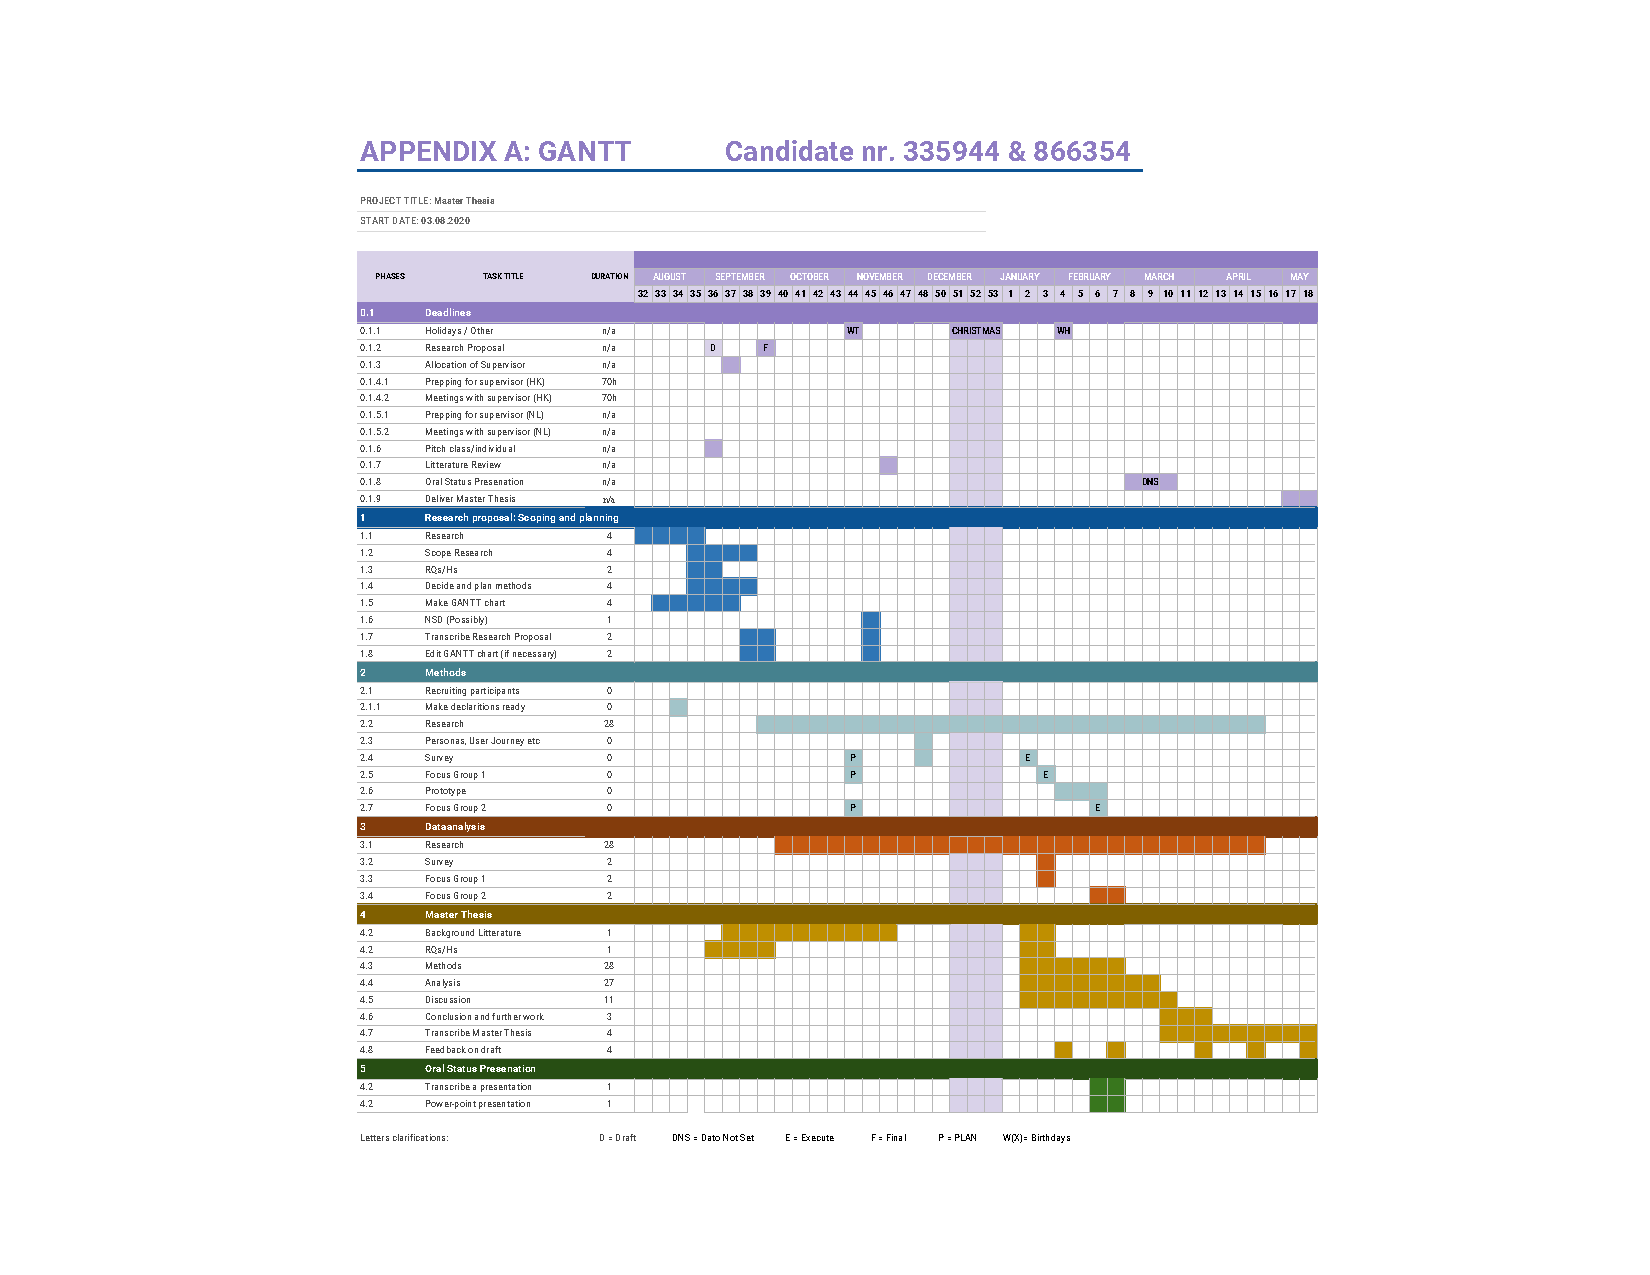
\includepdf[scale=1.5,pages=-]{Gantt.pdf}

\end{appendices}






\end{document}